% fig_ar_scheme.tex
% TR-36: AR scheme state machine
% States: NORMAL → FAULT_TRIP → DEAD_TIME → RECLOSE → (SERVICE_RESTORED | LOCK_OUT)
% Shows protection function available at each state

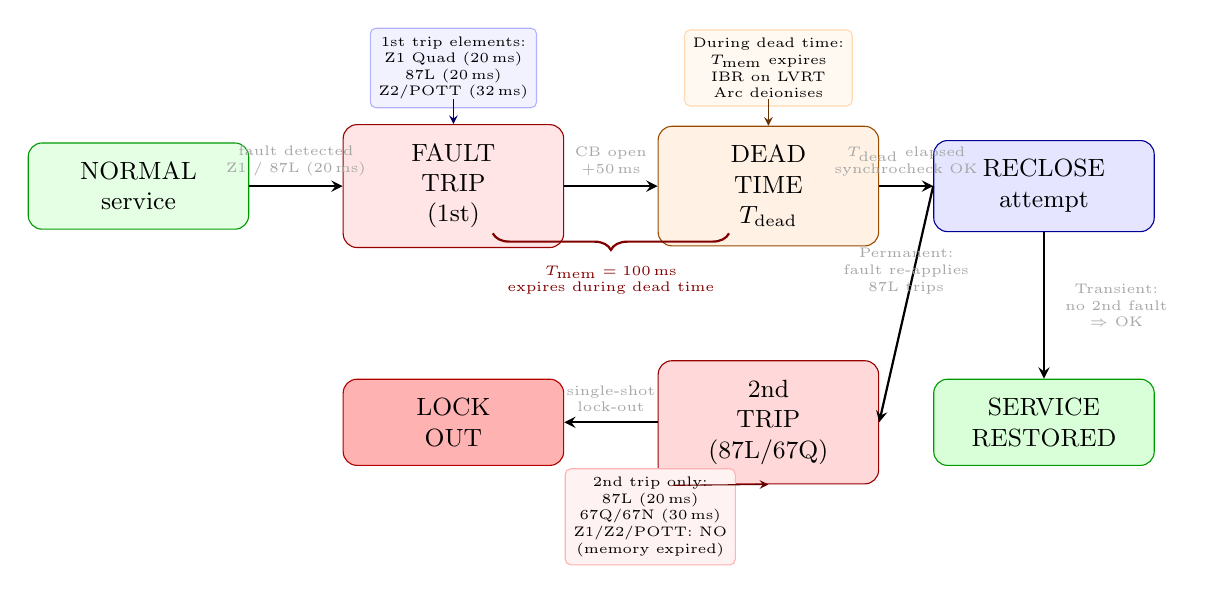
\begin{tikzpicture}[
  every node/.style = {font=\small},
  state/.style = {draw, rounded corners=5pt, inner sep=7pt, align=center,
                  minimum width=2.8cm, minimum height=1.0cm},
  arr/.style  = {->, >=stealth, thick},
  note/.style = {font=\tiny, align=center, text=gray!70},
]

%% ── States ────────────────────────────────────────────────────────────────────
\node[state, fill=green!10, draw=green!60!black]
  (normal) at (0, 0) {NORMAL\\service};

\node[state, fill=red!10, draw=red!60!black]
  (trip) at (4.0, 0) {FAULT\\TRIP\\(1st)};

\node[state, fill=orange!10, draw=orange!60!black]
  (dead) at (8.0, 0) {DEAD\\TIME\\$T_\mathrm{dead}$};

\node[state, fill=blue!10, draw=blue!60!black]
  (reclose) at (11.5, 0) {RECLOSE\\attempt};

\node[state, fill=green!15, draw=green!60!black]
  (restore) at (11.5, -3.0) {SERVICE\\RESTORED};

\node[state, fill=red!15, draw=red!60!black]
  (trip2) at (8.0, -3.0) {2nd\\TRIP\\(87L/67Q)};

\node[state, fill=red!30, draw=red!70!black]
  (lock) at (4.0, -3.0) {LOCK\\OUT};

%% ── Transitions ──────────────────────────────────────────────────────────────
% NORMAL → FAULT_TRIP
\draw[arr] (normal.east) -- (trip.west)
  node[midway, above, note] {fault detected\\Z1 / 87L (20\,ms)};

% FAULT_TRIP → DEAD_TIME
\draw[arr] (trip.east) -- (dead.west)
  node[midway, above, note] {CB open\\+50\,ms};

% DEAD_TIME → RECLOSE
\draw[arr] (dead.east) -- (reclose.west)
  node[midway, above, note] {$T_\mathrm{dead}$ elapsed\\synchrocheck OK};

% RECLOSE → SERVICE_RESTORED (transient)
\draw[arr] (reclose.south) -- (restore.north)
  node[midway, right=4pt, note] {Transient:\\no 2nd fault\\$\Rightarrow$ OK};

% RECLOSE → 2nd TRIP (permanent)
\draw[arr] (reclose.west) -- (trip2.east)
  node[midway, above, note] {Permanent:\\fault re-applies\\87L trips};

% 2nd TRIP → LOCK_OUT
\draw[arr] (trip2.west) -- (lock.east)
  node[midway, above, note] {single-shot\\lock-out};

%% ── Protection function annotations ─────────────────────────────────────────
% At first trip
\node[draw=blue!30, fill=blue!5, rounded corners=2pt,
      font=\tiny, inner sep=3pt, align=center]
  at (4.0, 1.5)
  {1st trip elements:\\Z1 Quad (20\,ms)\\87L (20\,ms)\\Z2/POTT (32\,ms)};
\draw[->, >=stealth, blue!40!black, thin] (4.0, 1.1) -- (trip.north);

% At dead time
\node[draw=orange!30, fill=orange!5, rounded corners=2pt,
      font=\tiny, inner sep=3pt, align=center]
  at (8.0, 1.5)
  {During dead time:\\$T_\mathrm{mem}$ expires\\IBR on LVRT\\Arc deionises};
\draw[->, >=stealth, orange!40!black, thin] (8.0, 1.1) -- (dead.north);

% At 2nd trip
\node[draw=red!30, fill=red!5, rounded corners=2pt,
      font=\tiny, inner sep=3pt, align=center]
  at (6.5, -4.2)
  {2nd trip only:\\87L (20\,ms)\\67Q/67N (30\,ms)\\Z1/Z2/POTT: NO\\(memory expired)};
\draw[->, >=stealth, red!40!black, thin] (6.8, -3.8) -- (trip2.south);

%% ── Memory window note ───────────────────────────────────────────────────────
\draw[red!50!black, thick, decorate,
      decoration={brace, amplitude=6pt, mirror}]
  (4.50, -0.60) -- (7.50, -0.60)
  node[midway, below=8pt, red!50!black, font=\tiny, align=center]
  {$T_\mathrm{mem}=100$\,ms\\expires during dead time};

\end{tikzpicture}
